\begin{figure*}[ht]
\begin{subfigure}{.5\textwidth}
  \centering
  % include first image
  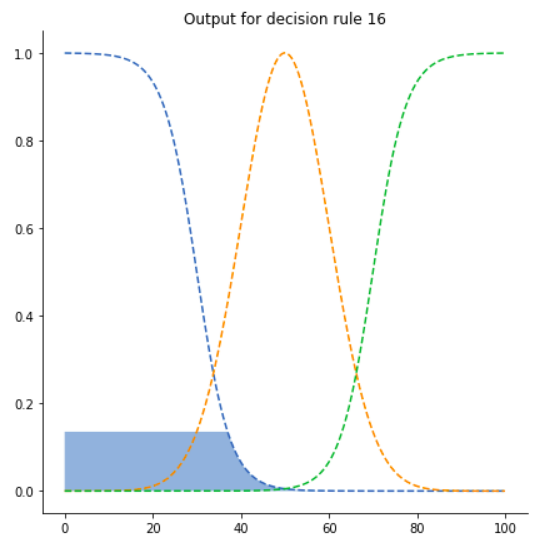
\includegraphics[width=.8\linewidth]{figures/first/min1.png}  
  \caption{Output for decision rule 16 with the T-norm minimum.}
  \label{fig:1min1}
\end{subfigure}
\begin{subfigure}{.5\textwidth}
  \centering
  % include second image
  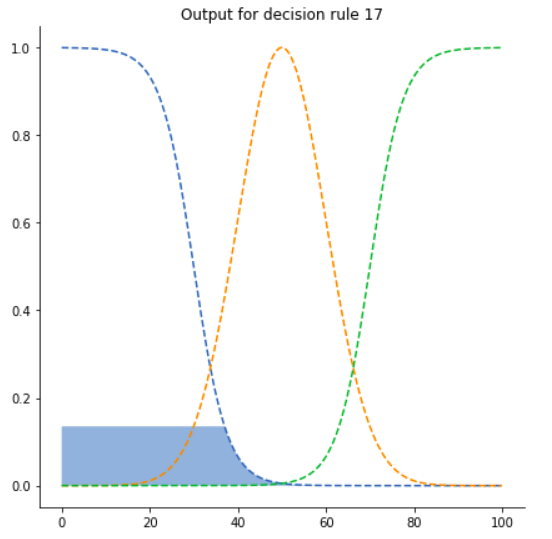
\includegraphics[width=.8\linewidth]{figures/first/min2.png}  
  \caption{Output for decision rule 17 with the T-norm minimum.}
  \label{fig:1min2}
\end{subfigure}
\begin{subfigure}{.5\textwidth}
  \centering
  % include second image
  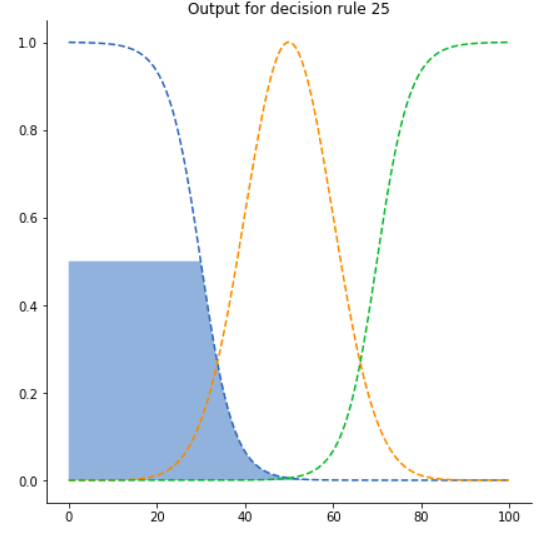
\includegraphics[width=.8\linewidth]{figures/first/min3.png}  
  \caption{Output for decision rule 25 with the T-norm minimum.}
  \label{fig:1min3}
\end{subfigure}
\begin{subfigure}{.5\textwidth}
  \centering
  % include second image
  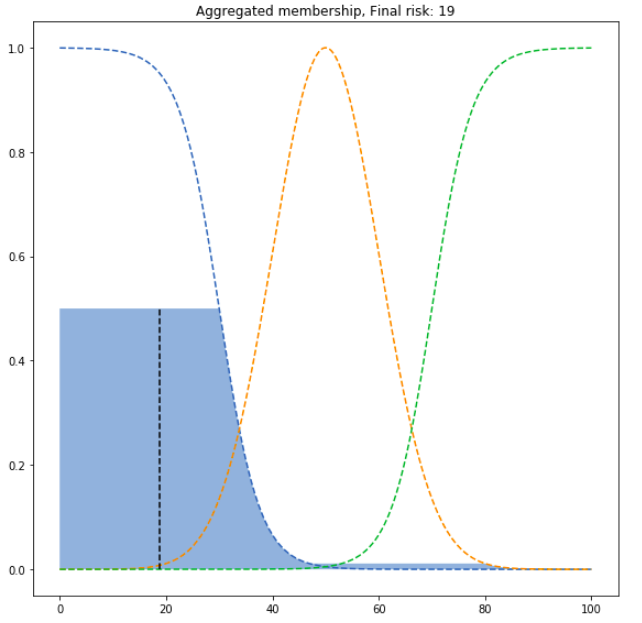
\includegraphics[width=.8\linewidth]{figures/first/min-centroid.png}  
  \caption{Final aggregation result with the centroid method for defuzzification.}
  \label{fig:1min-centroid}
\end{subfigure}
\begin{subfigure}{.5\textwidth}
  \centering
  % include second image
  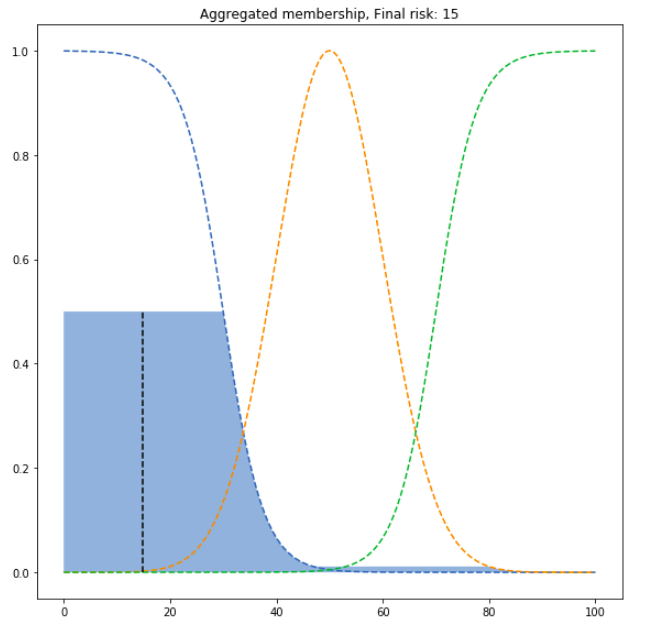
\includegraphics[width=.8\linewidth]{figures/first/min-mom.png}  
  \caption{Final aggregation result with the mean of maximum method for defuzzification.}
  \label{fig:1min-mom}
\end{subfigure}
\begin{subfigure}{.5\textwidth}
  \centering
  % include second image
  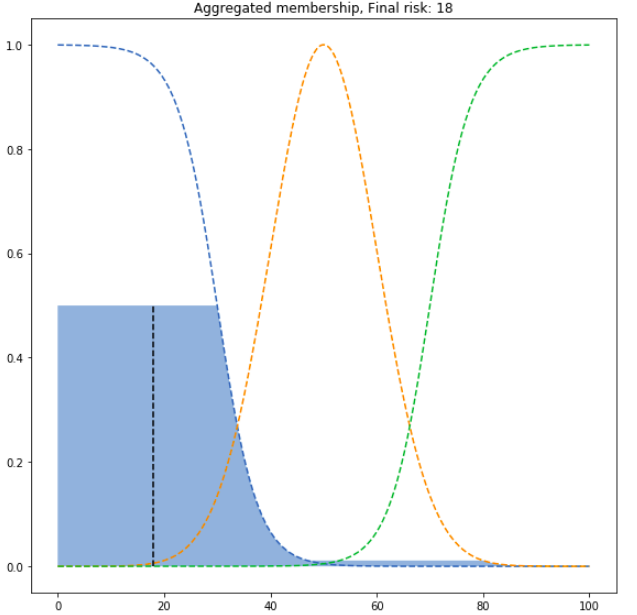
\includegraphics[width=.8\linewidth]{figures/first/min-bisector.png}  
  \caption{Final aggregation result with the bisector method for defuzzification.}
  \label{fig:1min-bisector}
\end{subfigure}
\caption{Results for test case 1 using the T-norm minimum.}
\label{fig:testcase1min}
\end{figure*}

\begin{figure*}[ht]
\begin{subfigure}{.5\textwidth}
  \centering
  % include first image
  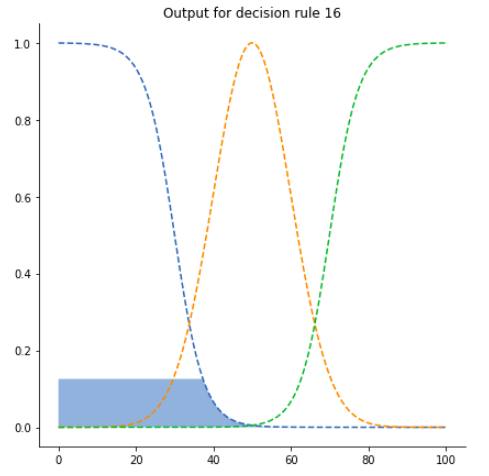
\includegraphics[width=.8\linewidth]{figures/first/prod1.png}  
  \caption{Output for decision rule 16 with the T-norm product.}
  \label{fig:1prod1}
\end{subfigure}
\begin{subfigure}{.5\textwidth}
  \centering
  % include second image
  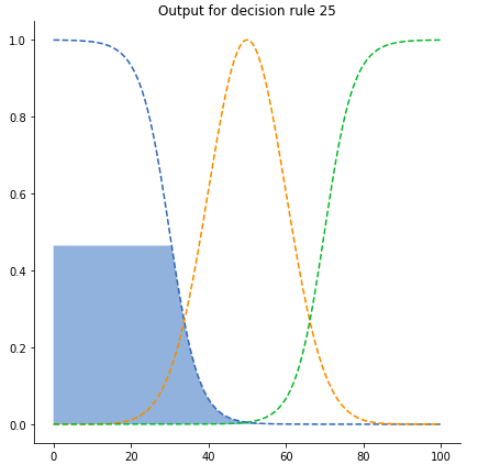
\includegraphics[width=.8\linewidth]{figures/first/prod2.png}  
  \caption{Output for decision rule 17 with the T-norm product.}
  \label{fig:1prod2}
\end{subfigure}
\begin{subfigure}{.5\textwidth}
  \centering
  % include second image
  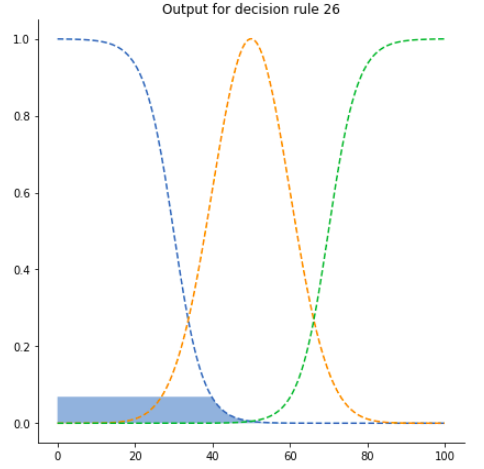
\includegraphics[width=.8\linewidth]{figures/first/prod3.png}  
  \caption{Output for decision rule 25 with the T-norm product.}
  \label{fig:1prod3}
\end{subfigure}
\begin{subfigure}{.5\textwidth}
  \centering
  % include second image
  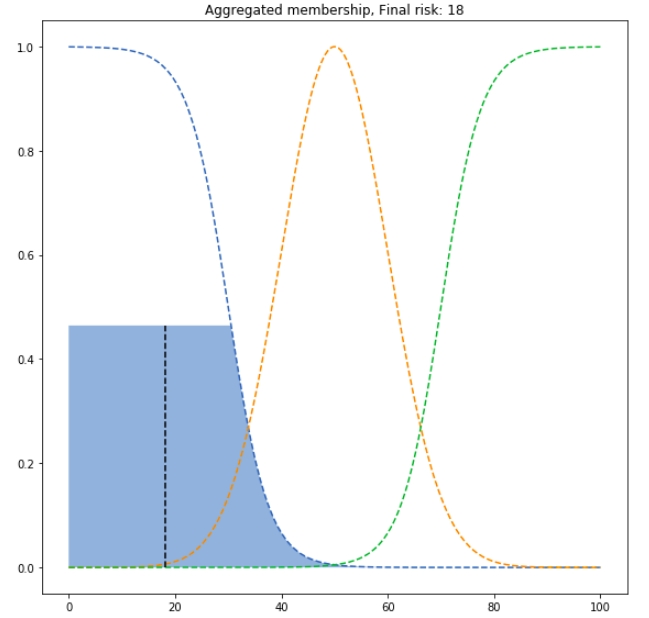
\includegraphics[width=.8\linewidth]{figures/first/prod-centroid.png}  
  \caption{Final aggregation result with the centroid method for defuzzification.}
  \label{fig:1prod-centroid}
\end{subfigure}
\begin{subfigure}{.5\textwidth}
  \centering
  % include second image
  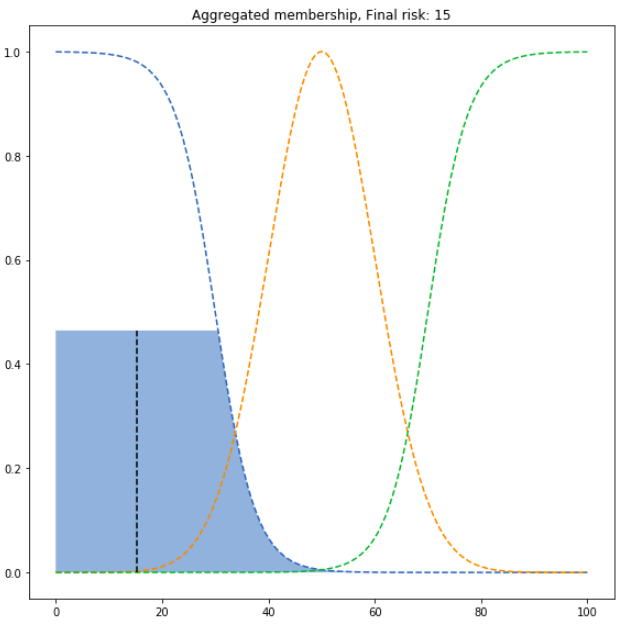
\includegraphics[width=.8\linewidth]{figures/first/prod-mom.png}  
  \caption{Final aggregation result with the mean of maximum method for defuzzification.}
  \label{fig:1prod-mom}
\end{subfigure}
\begin{subfigure}{.5\textwidth}
  \centering
  % include second image
  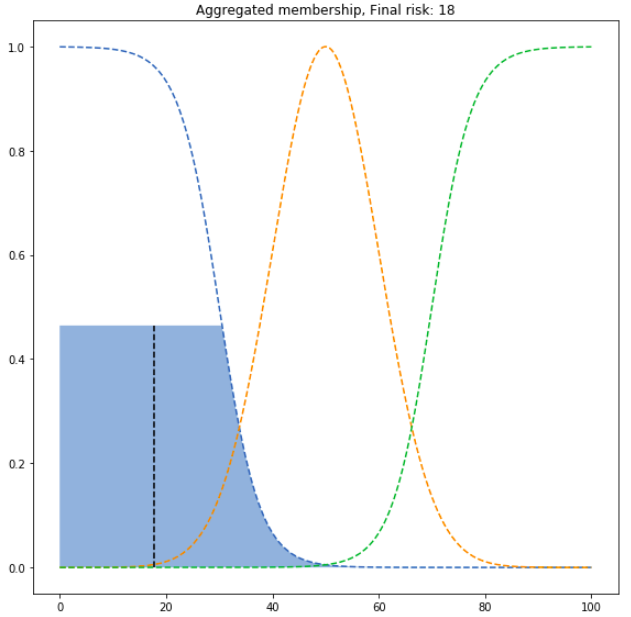
\includegraphics[width=.8\linewidth]{figures/first/prod-bisector.png}  
  \caption{Final aggregation result with the bisector method for defuzzification.}
  \label{fig:1prod-bisector}
\end{subfigure}
\caption{Results for test case 1 using the T-norm product.}
\label{fig:testcase1prod}
\end{figure*}